% Renato Bellotti, October 2018

\documentclass{beamer}

\usepackage{tikz}
\usepackage{enumitem}
\usepackage{tcolorbox}

\setbeamertemplate{navigation symbols}{}

%\newcommand{\UP}{1}
%\newcommand{\RIGHT}{2}
%\newcommand{\DOWN}{3}
%\newcommand{\LEFT}{4}

% (x, y) denotes the top left position of the arrow
% length, x, y, orientation
%\newcommand{\spin}[4][0.5]{
%    \ifthenelse{#4 = \UP}{
%        \draw[->] (#2, #3) -- (#2, #3 + #1);
%    }{}
%    \ifthenelse{#4 = \RIGHT}{
%        \draw[->] (#2, #3) -- (#2 + #1, #3);
%    }{}
%    
%    \ifthenelse{#4 = \DOWN}{
%        \draw[->] (#2, #3) -- (#2, #3);
%    }{}
%}
\newcommand{\up}[0]{$\uparrow$}
\newcommand{\down}[0]{$\downarrow$}

\newenvironment{mybox}{\begin{tcolorbox}[sharp corners=all, frame empty]}{\end{tcolorbox}}


\begin{document}

\begin{frame}{Multi-GPU accelerated multi-spin Monte Carlo simulations of the 2D Ising model}
\begin{tabular}{c c c}
    %\begin{tikzpicture}
%\spin{1}{1}{2}
%\end{tikzpicture}
%\documentclass{article}

%\usepackage{fancyhdr}

%\pagestyle{fancy}
%\fancyfoot{}

%%\newcommand{\UP}{1}
%\newcommand{\RIGHT}{2}
%\newcommand{\DOWN}{3}
%\newcommand{\LEFT}{4}

% (x, y) denotes the top left position of the arrow
% length, x, y, orientation
%\newcommand{\spin}[4][0.5]{
%    \ifthenelse{#4 = \UP}{
%        \draw[->] (#2, #3) -- (#2, #3 + #1);
%    }{}
%    \ifthenelse{#4 = \RIGHT}{
%        \draw[->] (#2, #3) -- (#2 + #1, #3);
%    }{}
%    
%    \ifthenelse{#4 = \DOWN}{
%        \draw[->] (#2, #3) -- (#2, #3);
%    }{}
%}
\newcommand{\up}[0]{$\uparrow$}
\newcommand{\down}[0]{$\downarrow$}

\newenvironment{mybox}{\begin{tcolorbox}[sharp corners=all, frame empty]}{\end{tcolorbox}}


%\begin{document}
{
\setlength{\tabcolsep}{8pt}
\renewcommand{\arraystretch}{1.2}

\begin{tabular}[b]{c c c c c}
    \up & \down & \down & \up & \down \\
    \down & \up & \down & \down & \down \\
    \up & \up & \down & \up & \down \\
    \up & \down & \up & \up & \down
    %$\uparrow$ & $\uparrow$ & $\uparrow$ & $\uparrow$ & $\uparrow$
\end{tabular}
}
%\end{document}

    \textbf{\huge{+}} &
    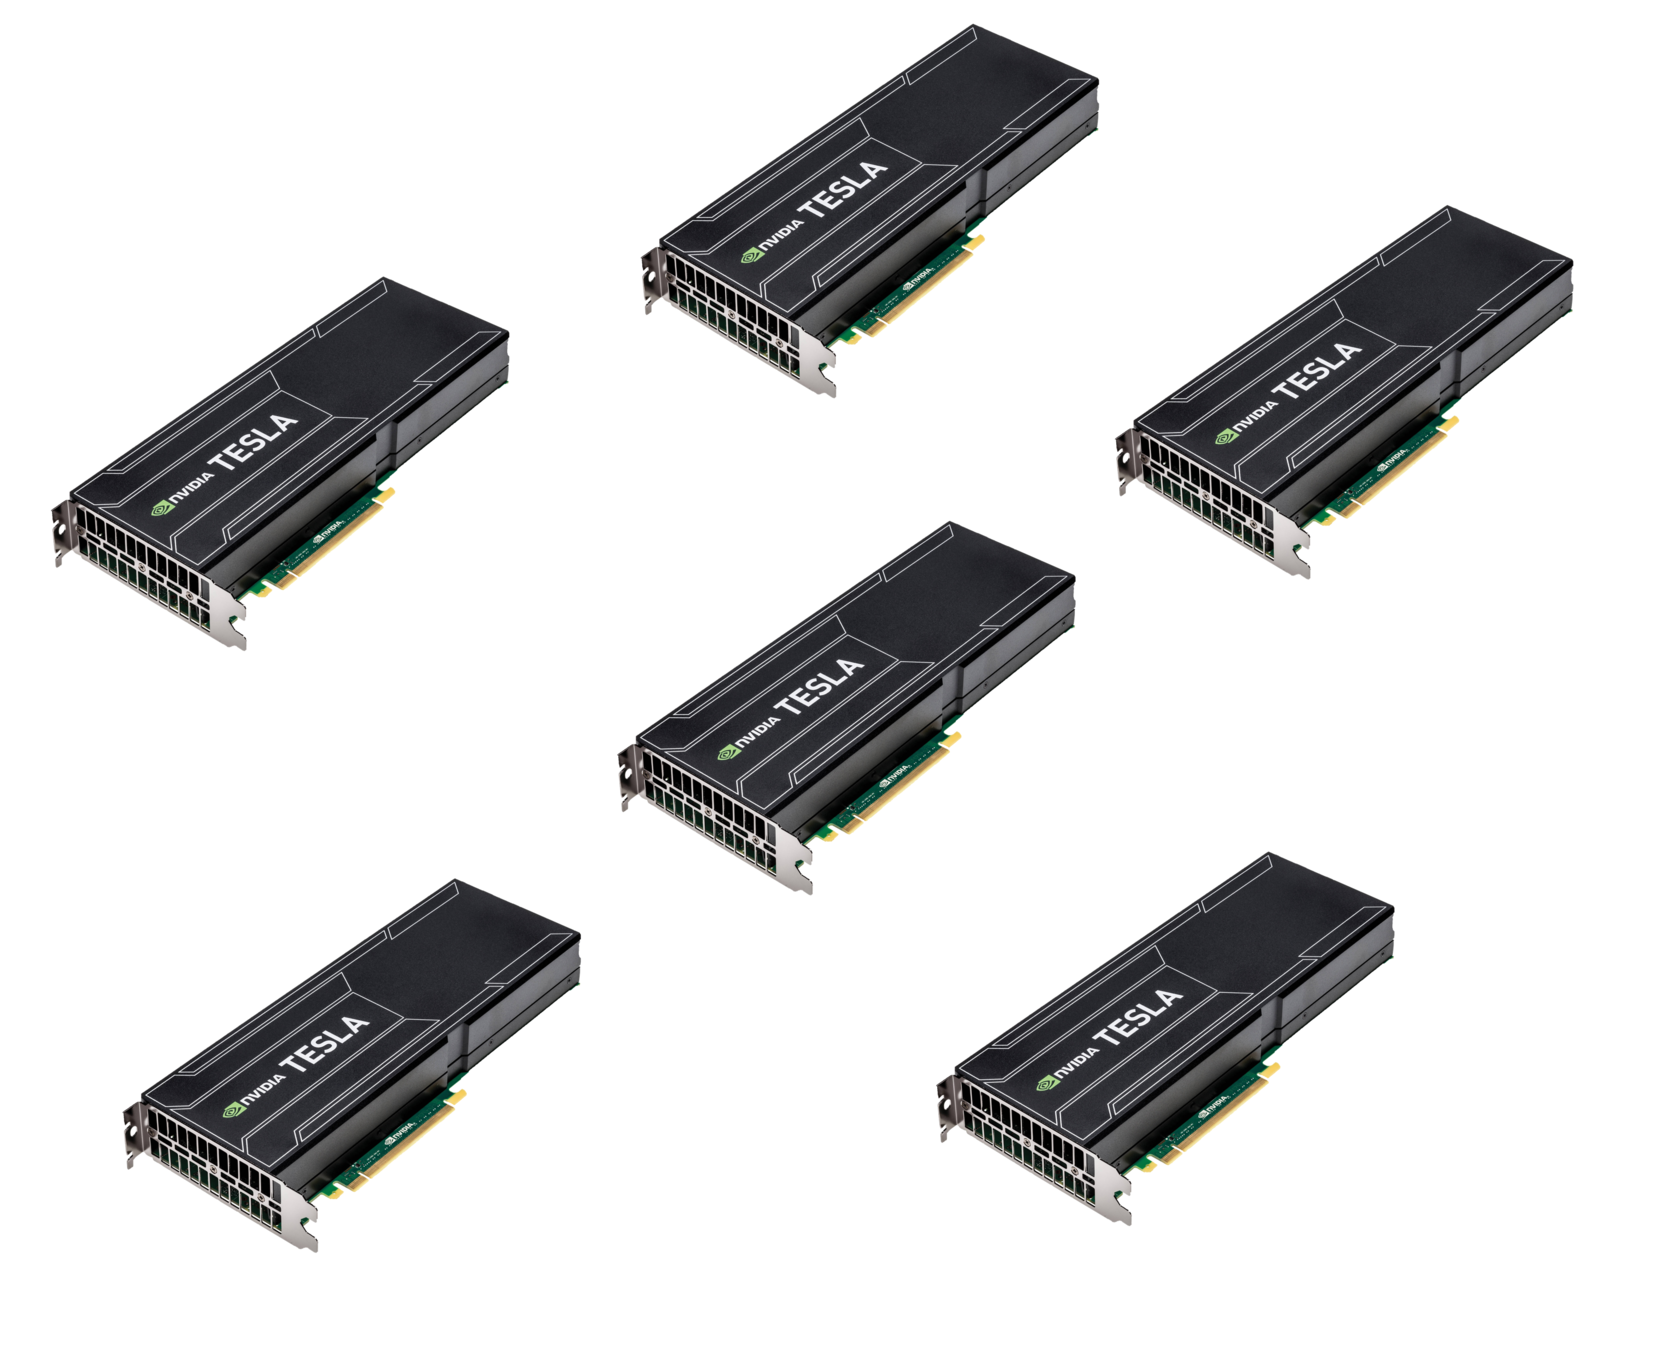
\includegraphics[keepaspectratio=true, width=0.2\paperwidth]{images/multi_gpu.png}
    \textbf{\huge{=}} &
    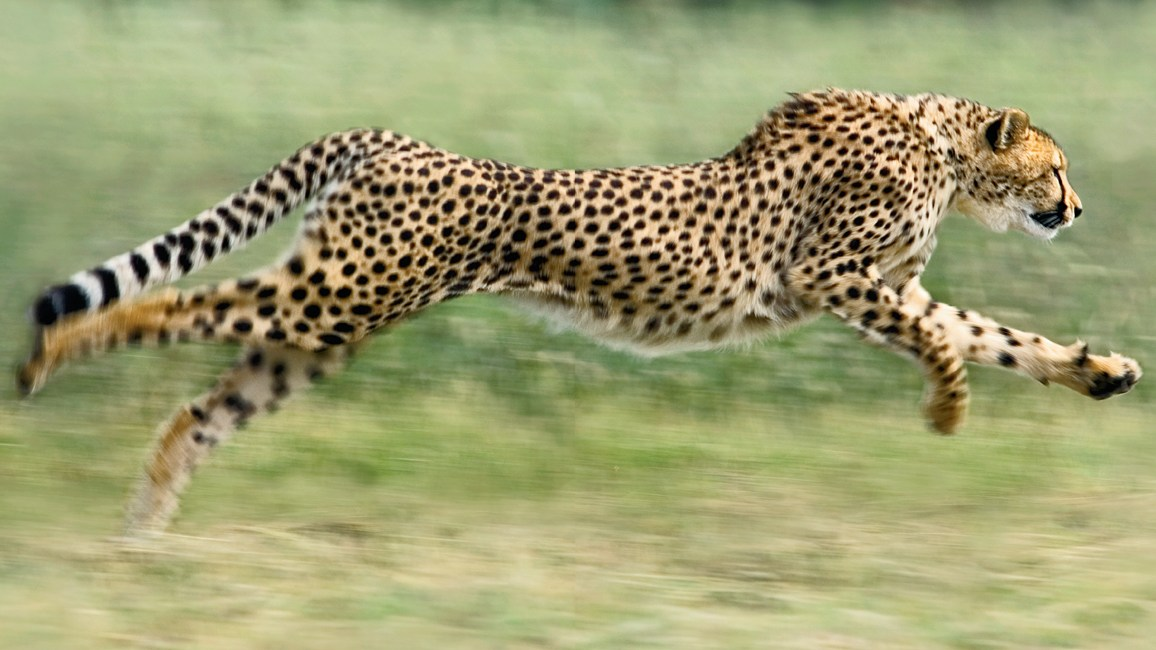
\includegraphics[keepaspectratio=true, width=0.2\paperwidth]{images/cheetah.jpg}
\end{tabular}
\end{frame}

\setcounter{framenumber}{0}
\setbeamertemplate{navigation symbols}{\insertframenumber}

\begin{frame}{What was done?}
\begin{columns}
    \begin{column}{0.5\paperwidth}
        \begin{itemize}
            \item \textbf{Ising model}
            \item \textbf{Metropolis algorithm:}\\
                Efficient sampling
        \end{itemize}
    \end{column} \pause
    \hfill
    \begin{column}{0.3\paperwidth}
        \begin{itemize}[itemsep=5mm]
            \item[] Single core CPU \pause
            \item[] Single GPU \pause
            \item[] Multpiple GPUs \pause
        \end{itemize}
    \end{column}
\end{columns}
\begin{mybox}
    How does it scale? Is it worth the effort?
\end{mybox}
\end{frame}

\end{document}
